\section{Image Segmentation}\label{sec:segmentation}
%\url{https://en.wikipedia.org/wiki/Image_segmentation#Trainable_segmentation}

%Segmentation is one of the most often automated medical imaging task~\autocite{MaierHein2018}.
In 2018, 70~\% of all biomedical image processing algorithms tried to solve the problem of image segmentation~\autocite{MaierHein2018}.
Segmentation is the process of partitioning images into multiple semantic sets of pixels (segments), for example to exactly locate objects within the image~\autocite{Szeliski2021}.
In the biomedical context, this could be outlining tumour boundaries, differentiating organs, vessels, and bones, locating metastases, or simply validating the position of implants.

\begin{figure}[!htb]
    \centering
    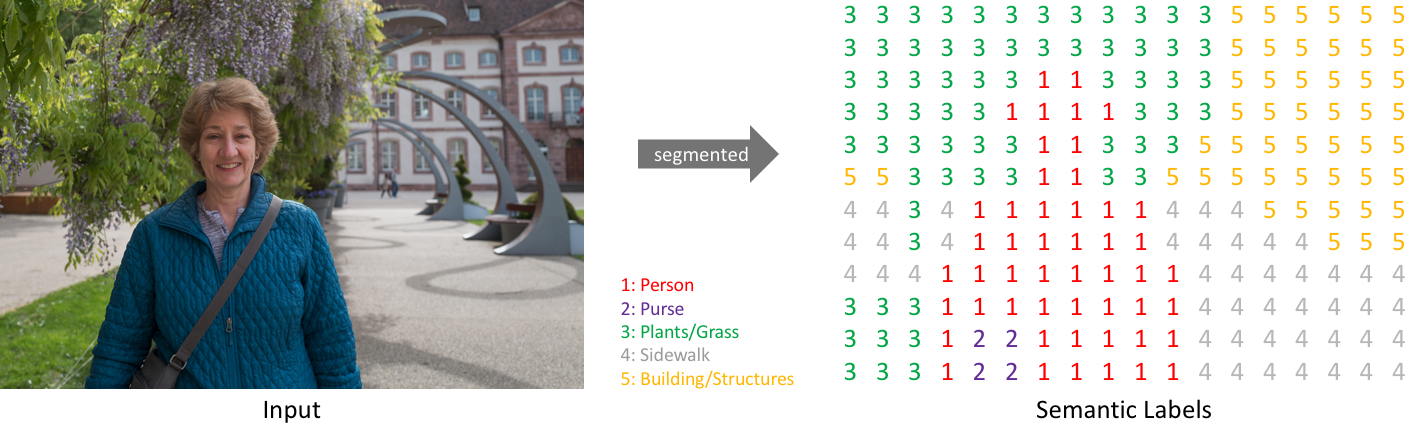
\includegraphics[width=\textwidth]{pictures/semantic-labels}\\
    \caption[Segmentation Map: Image and Labels]{Visualisation of an image and its segmentation map, containing the class labels of the pixels. For simplicity, a lower resolution segmentation map is shown. In reality, the resolutions match each other. Figure from~\autocite{Jordan2018}.}
    \label{fig:semantic-segmentation}
\end{figure}

%Definition
Segmentation is done by assigning a class label (usually an integer) to each pixel of an image.
These labels can be collected in a segmentation map of the same size as the image, as seen in \autoref{fig:semantic-segmentation}.
%classes of segmentation
Generally, segmentation is differentiated into semantic and instance segmentation.
In semantic segmentation, the same class is assigned to each object of the same type.
So, objects of the same class have the same label.
Instance segmentation differentiates between objects of the same class.~\autocite{Szeliski2021}

%used data and accompanying problems
Especially in scientific image processing, segmentation is a major challenge, since often diminutive structures are of interest and image quality is limited and highly variable, as imaging needs to be non-destructive and is often done in-vivo.


\subsection{Imaging Methods} \label{subsec:3d-imaging-data}
Today, two modalities are mainly used to generate 3D images of scientific samples without destroying them in the process: \glsfirst{ct} and \glsfirst{mrt}~\autocite{Ganguly2010}.
\gls{ct} utilises X-rays to generate an image of a sample, while \gls{mrt} is based on magnetic resonance of atoms in the body~\autocite{Pandit2014,Bercovich2018}.
Generally speaking, \gls{mrt} is better at differentiating soft tissues, while \gls{ct} is better suited to resolve bone structures, since it relies on X-rays, which are density dependent~\autocite{Bercovich2018}.
Additionally, \glspl{ct} can accomplish higher resolutions, especially when using specialised methods like \glsfirst{mct} or \glsfirst{srmct}~\autocite{Pandit2014}.

\subsubsection{Computed Tomography}\label{subsubsec:computed-tomography}
In a \gls{ct}, samples are rotated through the beam (or, in the case of patients, the beam is rotated around the sample) and the 2D intensity pattern of the emerging beam is recorded, indicating the distribution of materials in the sample~\autocite{Bercovich2018}.
Millions of 2D pictures are taken from various positions and angles and are then used to reconstruct a 3D image of the sample by means of reconstruction algorithms (see~\autoref{subsec:data-pre-processing}).
During reconstruction, noise and artifacts from scanning can often be partially removed, but the remainders impede data quality and thus segmentation results~\autocite{Vidal2005}.

%SRµCT
Four main properties have been found to significantly enhance data quality in \glspl{ct}: parallel geometry, monochromaticity, high beam intensity and the propagation phase approach~\autocite{Tafforeau2006}.
All of these properties can be utilised in \glsfirst{srmct}.
The parallel geometry of a synchrotron, where all beams travel parallel instead of conical (as in a traditional \gls{ct}), leads to a much more exact reconstruction.
In addition, the high-energy beams derived from an electron synchrotron make it possible to filter the beam to use monochromatic X-rays, which prevent artifacts from beam hardening (brightening of sample borders and linking of dense structures)\footnote{Beam hardening occurs, because low-energy beams are absorbed more than high-energy beams (thus creating a ‘harder’ beam), generating artifacts, which need to be managed on a case-by-case basis after reconstruction.}.
The high beam intensity found in \gls{srmct} also leads to shorter exposure times (fractions of a second per slice) and thus shorter measuring times with very good resolutions.~\autocite{Tafforeau2006}

In summary, the advantage of \gls{srmct} in comparison to \gls{ct} is the beam intensity: in the former, it is high enough to use monochromatic X-rays, which are able to resolve even finer structures.
And so \gls{srmct} has become one of the most valuable tools in scientific studies.
However, two of the major problems of \gls{srmct} are availability and cost. 
There are only a few synchrotrons globally that reach sufficient beam intensity and so beamline-time is not easy to get.\footnote{Due to a collaboration with Hereon, who operates the Petra III beam lines at \gls{desy}, availability of \gls{srmct} data is not a problem in this study.}

\subsubsection{Magnetic Resonance Tomography}\label{subsubsec:magnetic-resonance-tomography}
\gls{mrt} is not based on passive absorption spectra, but on emissions from protons within the sample.
First, a fixed magnetic field is produced around the sample.
Then, radio frequency pulses are used to excite protons within the sample.
Once the protons relax back to a resting state, they emit a signal that is captured to create an image.~\autocite{Bercovich2018}

\gls{mrt} is superior to CT in soft tissue contrast and is used in nearly all medical domains, as it is often faster and does not use ionising radiation which is harmful in high doses.
Thus, it has become the main tool in oncology and examinations of the heart and brain.~\autocite{Bercovich2018}

\subsection{Data Pre-Processing}\label{subsec:data-pre-processing}
%data preparation
Before images can be used for segmentation, they have to be reconstructed from the 2D absorption spectra (in case of \gls{ct}) or emitted signal maps (in case of \gls{mrt}).
This is done by using specialised software, which also removes artifacts from scanning.
Additionally, images are re-sampled to achieve an even voxel\footnote{A voxel is a three-dimensional pixel.} spacing on all three axis, and normalised to reduce noise and get comparable data sets, not biased by their absolute voxel values~\autocite{Rorden2012}.
In the case of \gls{mrt}-data, normalisation is done on a per-image basis as voxel values are relative.
For \gls{ct}-data, normalisation may be done globally over all data sets, since voxel values are quantitative and reflect physical properties of the data set~\autocite{Isensee2019}.


\subsection{Segmentation Techniques} \label{subsec:problems-in-segmentation}
Traditionally, image segmentation was done with feature-based methods, which rely on properties like pixel value, or gradients (e.g.~watershed method, graph cut techniques or region growing), which need to be defined and selected arbitrarily by a human~\autocite{Kar2021}.
Due to the nature of medical images, they often suffer from low contrast, high spatial variability and scanning artifacts.
Thus, these traditional algorithms are often inaccurate, time-consuming and a lot of manual corrections needs to be done.

In recent years however, deep learning techniques were successfully used to automatically segment images, often even outperforming manual segmentation done by human experts in accuracy and in speed~\autocite{Antonelli2022}.
Deep learning techniques have the ability to improve the accuracy of the model automatically through experience~\autocite{Mitchell1997}, without being explicitly programmed to do so, thus they have the potential to be faster while requiring less human intervention.

For image processing, and even live video segmentation one of the most promising unsupervised deep learning algorithms of the last years is \gls{stego}, a transformer-based architecture, which was found to perform better than the current state-of-the art for unsupervised segmentation~\autocite{Hamilton2022}.
In this study, \gls{stego} will be adapted to be used with high-resolution scientific imaging data.
